\section{Configuration Spaces}
\subsection{Configuration Spaces of Linkages}
Let's focus on the space of embeddings of a linkage. The if there are $n$ vertices of a linkage, 
\textit{configuration space} of a linkage is said to be a vector space of dimension $2 n$ 
where edge length is preserved.  
\begin{figure}[!h]
\begin{center}
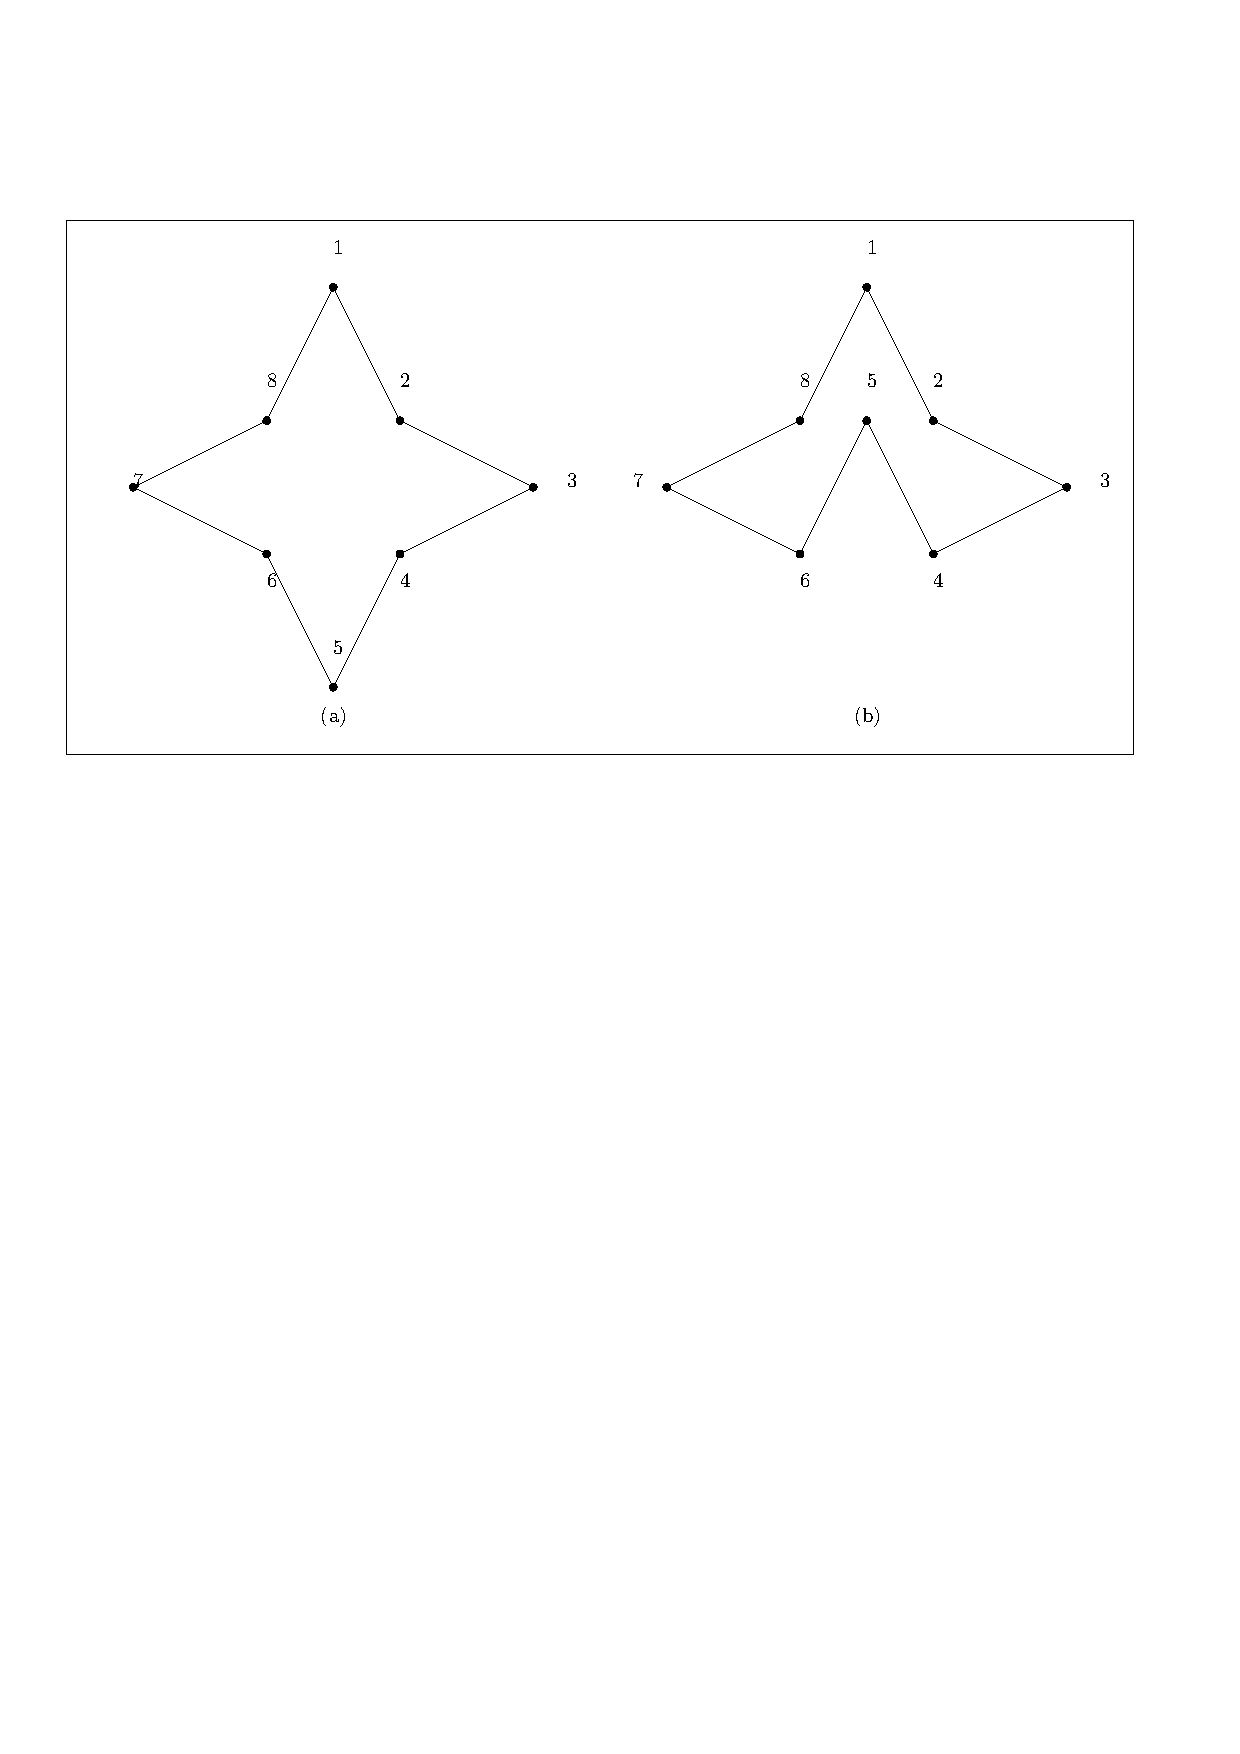
\includegraphics[scale=.75]{graphics/twoEmbeddingsOfSameLinkage.pdf}
\end{center} 
\caption{(a) and (b) show a linkage in two embeddings.}
\label{fig:configuration-3}
\end{figure}
A \textit{configuration space} for a linkage $G$ and corresponding proper embedding, $L_1$ is said 
to be for any other proper embedding of a linkage $G$, $L_2$, such that the lengths 
of every edge of $G$ is preserved between the two embeddings, i.e.: 
$$l\left( \left(u,v\right) 
\right) = \left\vert 
L_1(u) - L_1(v) \right\vert = \left\vert L_2(u) - L_2(v) \right\vert$$
Equivalent embeddings include translations and rotations about the center of mass on $L(V)$.  We 
further our embeddings by requiring that one vertice is pinned to the point of origin on the plane 
as well as a neighboring vertex.
%insert index here
\subsection{Configuration Spaces of Polygonal Linkages}
%Show example an example of a locked linkage and locked polygonal linkage.

% To describe the types of motion that we are interested in linkages we must define the graph 
% isomorphism.  Two graphs $G=(V_1,E_1)$ and $G_2 = (V_2,E_2) $, a bijection $f: V_1 \mapsto V_2$ 
% such that for any two vertices $u,v \in V_1$ that are adjacent, i.e. $(u, v) \in E_1$, if and only 
% if $(f(u),f(v)) \in E_2$. 
\begin{table}[!ht]
\begin{center}
$$\begin{array}{|c|c|c|}\hline
\text{Graph}&\text{Vertices}&\text{Edges}\\\hline
G_1&\left\lbrace a,b,c,d,e \right\rbrace & \left\lbrace (a,b),(b,c),(c,d),(d,e),(e,a) \right\rbrace 
\\\hline
G_2&\left\lbrace 1,2,3,4,5 \right\rbrace & \left\lbrace (1,2),(2,3),(3,4),(4,5),(5,1) \right\rbrace 
\\\hline
\end{array} $$
\caption{Two graphs that are isomorphic with the alphabetical isomorphism $f(a)=1$, $f(b)=2$, $f(c) 
= 3$, $f(d)=4$, $f(e)=5$.}
\end{center} 
\label{table:configuration-1}
\end{table} 
% show an example of polygonal linkages
\begin{figure}[!h]
\begin{center}
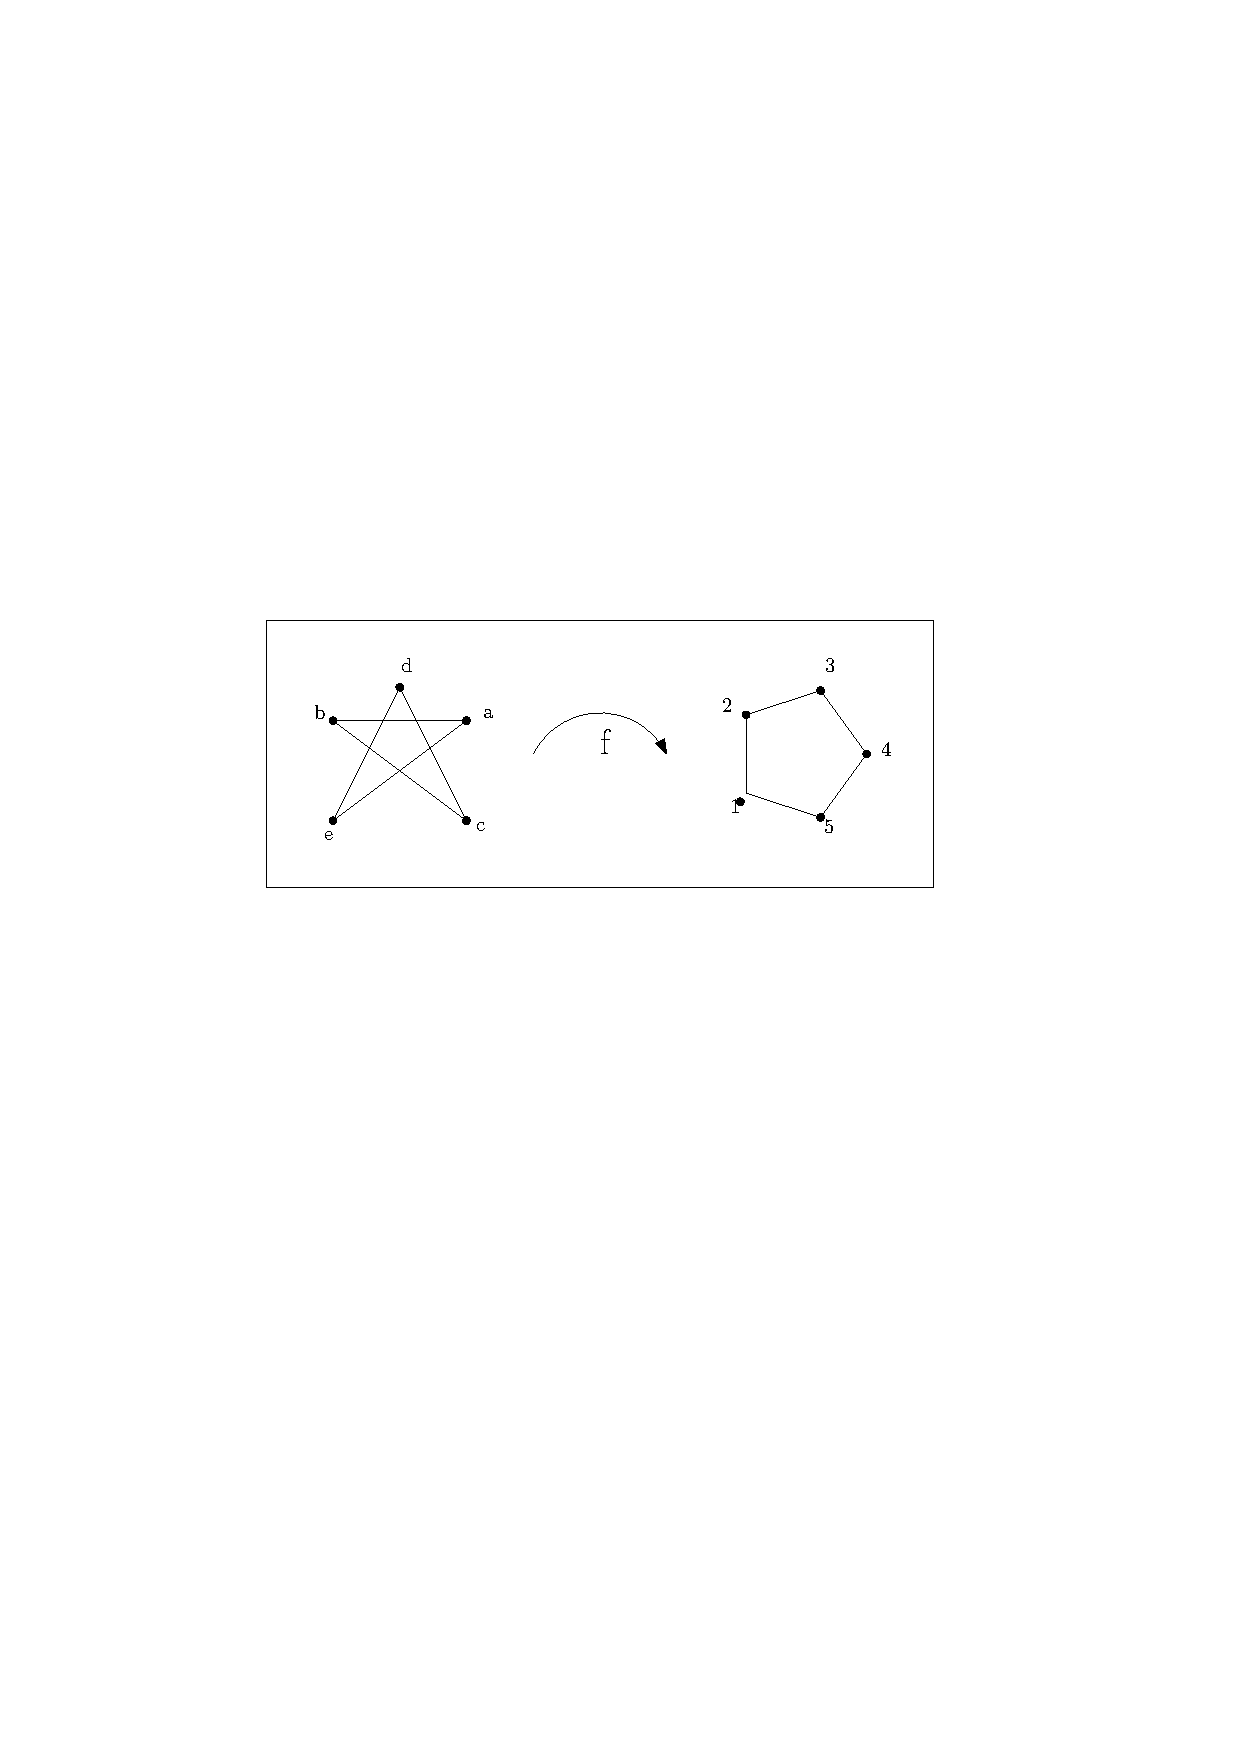
\includegraphics[scale=1]{graphics/graphIsomorphismExample.pdf}
\end{center} 
\caption{This figure depicts the graph isomorphism shown in Table 
(\ref{table:configuration-1}) between 
$V_1$ and $V_2$ in the plane.}
\label{fig:configuration-3}
\end{figure}
Next we add restrictions to our graph isomorphisms to narrow our focus:
\begin{itemize}
\item[\rn{1}] We focus on isomorphisms for planar graphs and or polygonal linkages, simple planar 
graphs, and
\item[\rn{2}] the isomorphism preserves edge lengths (polygonal area), e.g. $d(u,v) = d(f(u),f(v))$.
\end{itemize}  


















\subsubsection{Confining Linkages to a Restricted Space Within a Configuration Space}
So we've covered the idea of linkages within a plane; now let's constrain the plane to a strip and have a linkage that is a \textit{polygon}, i.e. a linkage that forms a closed chain (e.g. Table \ref{table:linkage-1}), hugging the boundaries of the strip:
\begin{figure}[h]
\begin{center}
  ~ %add desired spacing between images, e. g. ~, \quad, \qquad etc.
    %(or a blank line to force the subfigure onto a new line)
  \begin{subfigure}[b]{0.49\textwidth}
	  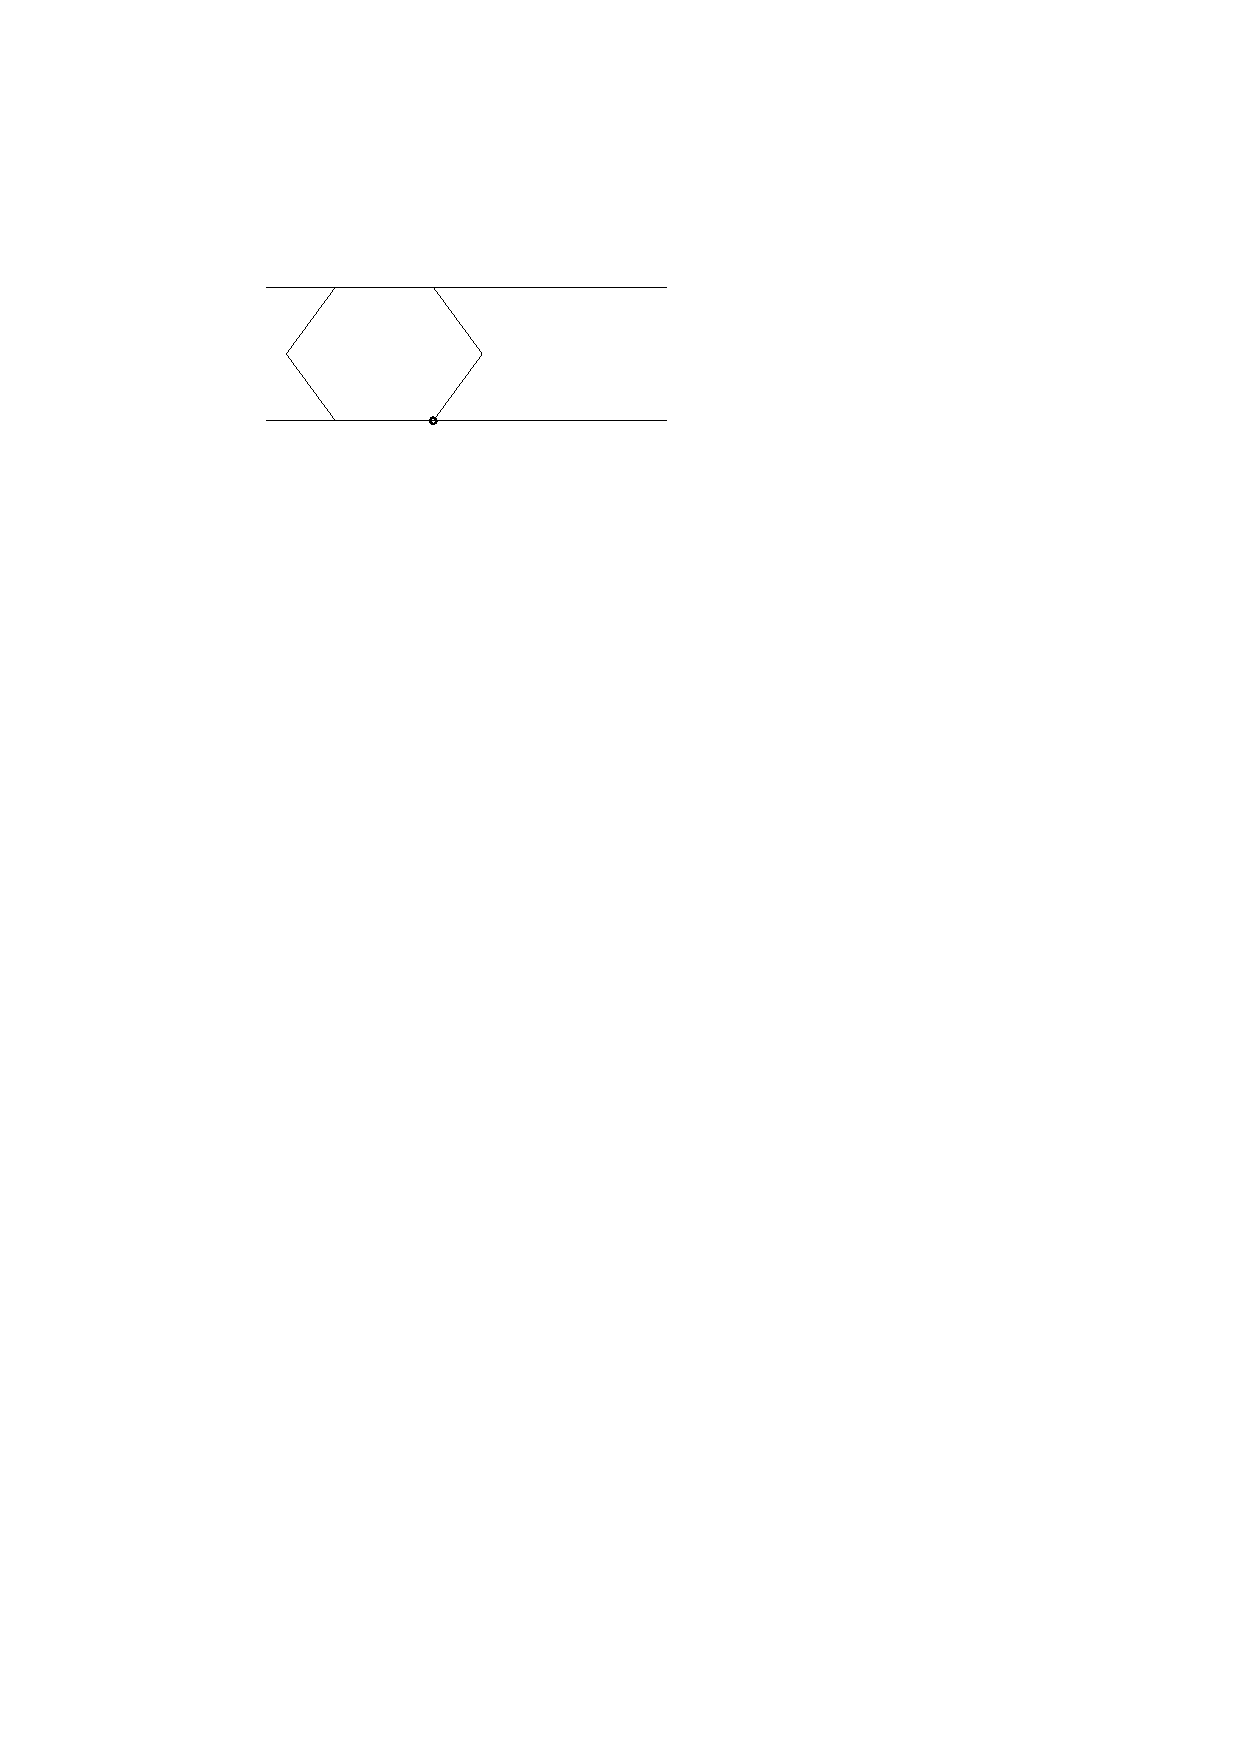
\includegraphics[width=\textwidth]{graphics/hexagonInChannelWithPinnedJointRight.pdf}
	  \caption{A bounded hexagon that resides in a channel with a pinned vertex}
	  \label{fig:linkage-1-1}
  \end{subfigure}
  \begin{subfigure}[b]{0.49\textwidth}
	  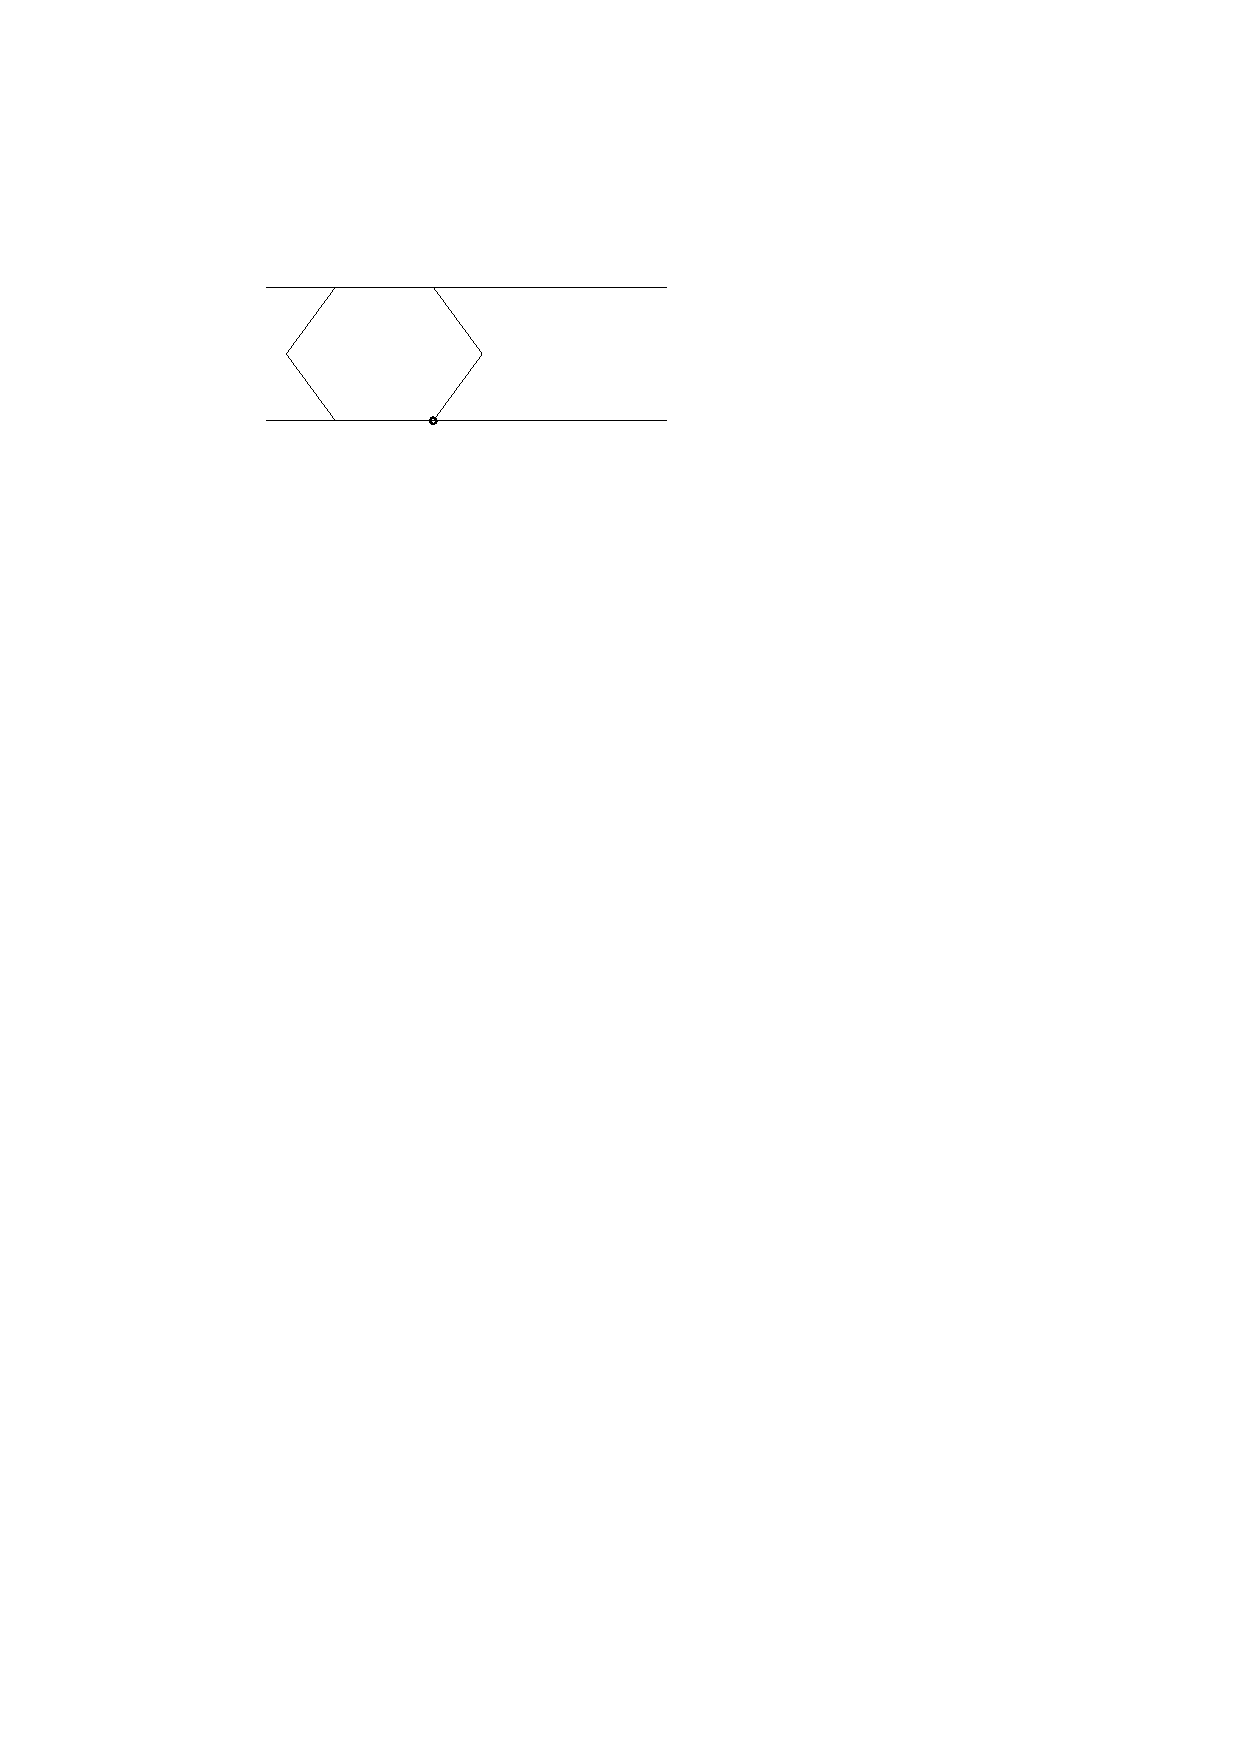
\includegraphics[width=\textwidth]{graphics/hexagonInChannelWithPinnedJointLeft.pdf}
	  \caption{The second realization of the hexagon residing in a channel with a pinned vertex.}
	  \label{fig:linkage-1-2}
  \end{subfigure}
\end{center} 
\caption{Due to the strip in the plane that the hexagon is bounded within the configuration space is limited to just two realizations.}\label{fig:linkage-1}
\end{figure}
So here we have a linkage whose conifguration space is limited to just two realizations.  With just two realizations, we can assign a binary value to them and have the linkage act as a boolean variable.  We will revisit this concept when we cover satisfiability problems later on in the paper.
\begin{figure}[h]
\begin{center}
  ~ %add desired spacing between images, e. g. ~, \quad, \qquad etc.
    %(or a blank line to force the subfigure onto a new line)
  \begin{subfigure}[b]{0.49\textwidth}
	  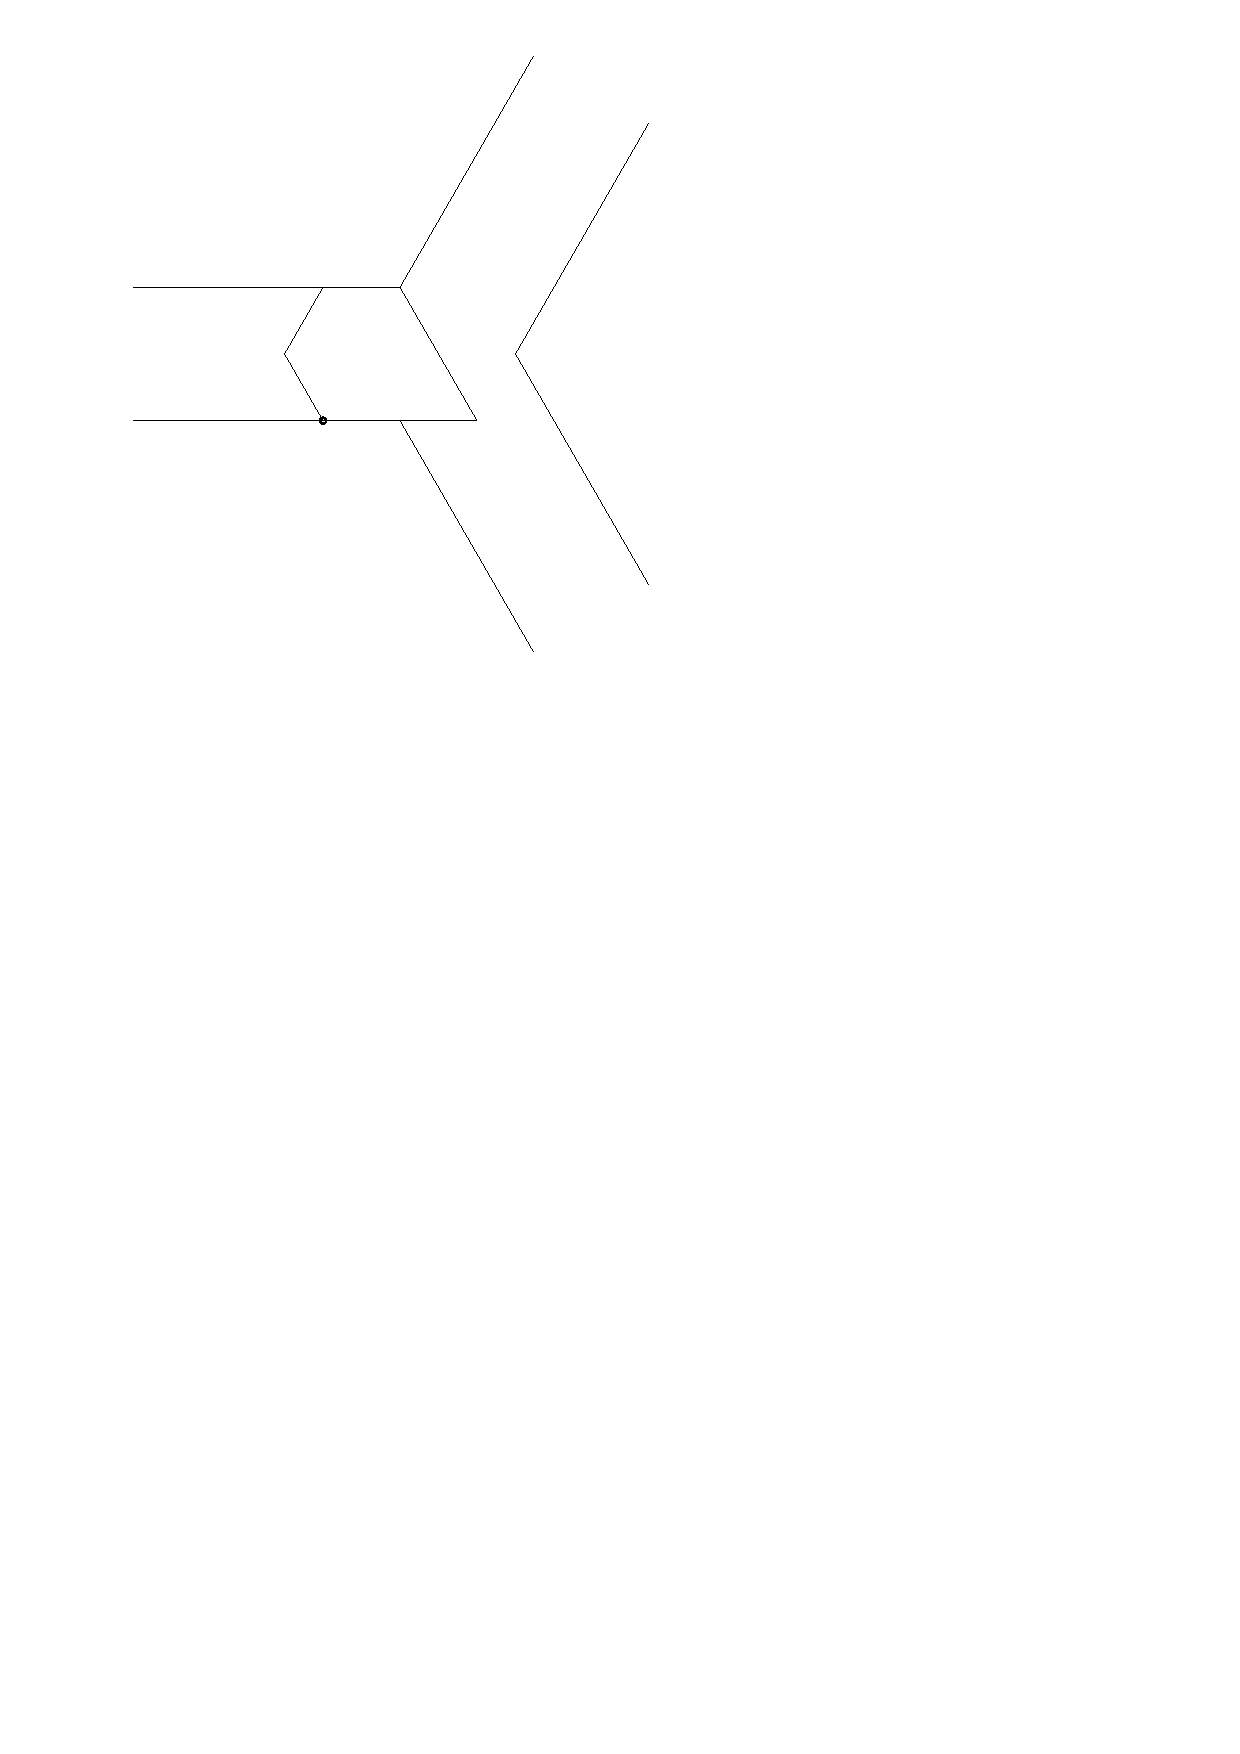
\includegraphics[width=\textwidth]{graphics/switchTerminalFinalized2.pdf}
	  \caption{A pentagon that is pinned in a channel junction that is formed by the sides of 3 large regular hexagons. It has two possible configurations, much like that of \ref{fig:linkage-1}}
	  \label{fig:linkage-2-1}
  \end{subfigure}
  \begin{subfigure}[b]{0.49\textwidth}
	  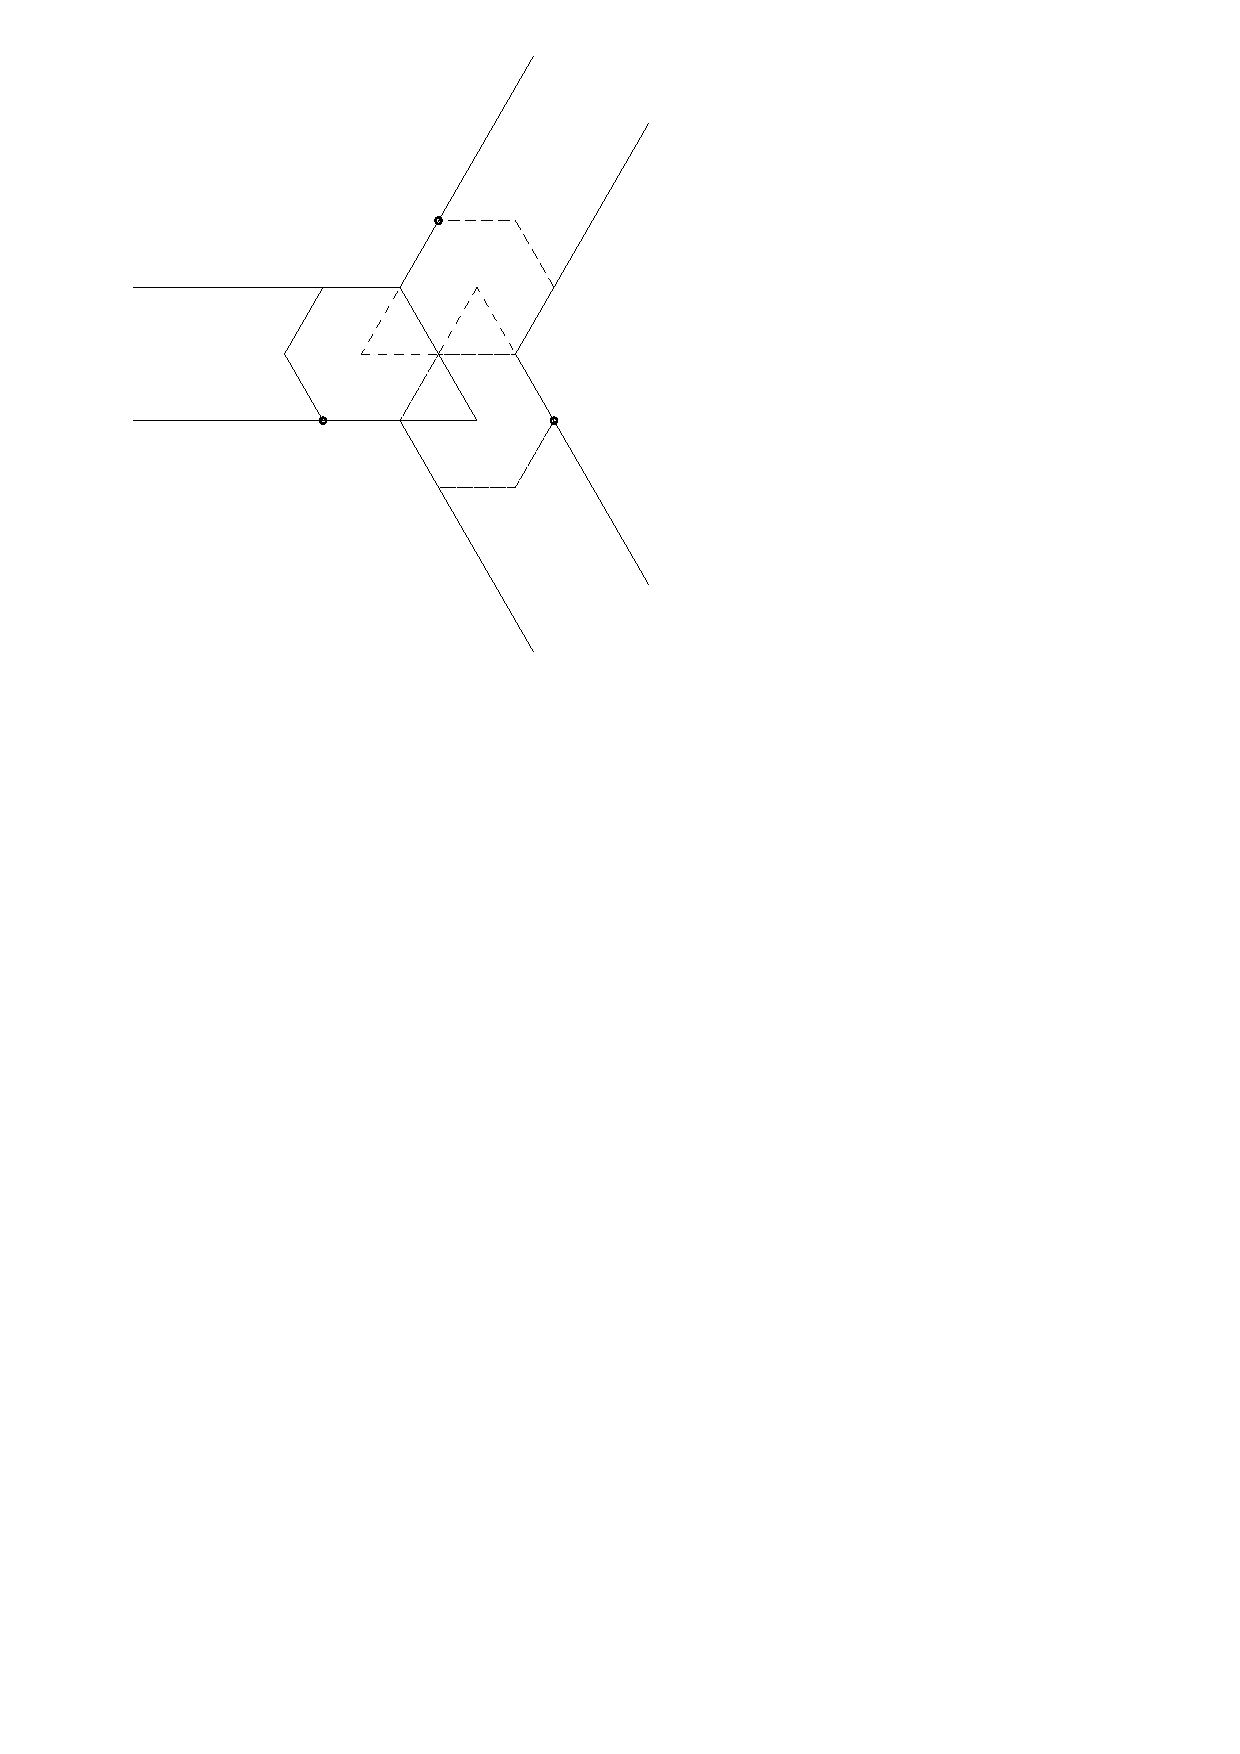
\includegraphics[width=\textwidth]{graphics/switchTerminalFinalized3.pdf}
	  \caption{A pinned pentagon residing in a channel junction that is formed by the sides of 
3 large regular hexagons with 2 dashed pentagons intersecting it.}
	  \label{fig:linkage-2-2}
  \end{subfigure}
\caption{Suppose the channel formed is a junction of three regular hexagons.  The polygon partially 
residing in the junction is a regular hexagon with an equalateral triangle appended at an edge.  
This polygon would prevent other polygons (i.e. the dashed polygons) of the same shape residing in 
the center of the channel without intersection. This demonstrates that a the configuration space 
within a multichannel environment can have concurrency issues, i.e. some configurations cannot be 
realizable.}
\end{center} \label{fig:linkage-2}
\end{figure}\newpage
Expanding upon the idea of \ref{fig:linkage-1}, forming channels with junctions as shown in Figure 
\ref{fig:linkage-2} can be formed as such by evenly spacing the edges of a hexagonal lattice.  
Visually, it is shown that only one of three possible pentagons can reside in the channel at one 
time.  By asserting certain conditions on the lattice, and extending the problem to a greater region 
of a hexagonal lattice, we will be able to pose a realizability problem of whether a configuration 
$\mathcal{A}$ can be reconfigured to $\mathcal{B}$ by switching pentagons without violating 
overlapped polygon conditions.
%Radius of regular polygons 
\newdimen\R
\R=3cm
% \begin{figure}[h] 
% \begin{center}
% \begin{tikzpicture}
% \begin{scope}
% \filldraw[pattern=hexagons]  (0:\R) \foreach \x in {60,120,...,359} {
%                 -- (\x:\R)
%             }-- cycle (90:\R);
% \end{scope}
% \end{tikzpicture}
% \caption{A hexagonal lattice contained in a hexagon.}
% \label{fig:lattice}
% \end{center}
% \end{figure}
\newpage

% \begin{definition}[Graph]\label{def:linkages-2}
% An ordered pair $G = (V, E)$ comprising a set $V$ of vertices or nodes together with a set $E$ of edges or lines
% \end{definition} 
% \begin{definition}[Linkage]\label{def:linkages-1}
% A collection of fixed-length 1D segments joined at their endpoints to form a graph.
% \end{definition} 
% A linkage can be thought of as a type of path-connected graph, i.e. the segments of a linkage are the edges of a graph, and the endpoints of the segments are the vertices. For this paper, we restrict our self to linkages that are simple planar graphs, i.e. a linkage that:
% \begin{itemize}
% \item[\rn{1}] does not have multiple edges between any pair of vertices,
% \item[\rn{2}] does not have edges that cross, or
% \item[\rn{3}] have loops (i.e. $(v,v) \in E$).
% \end{itemize}  
% \begin{definition}[Cycle]\label{def:linkages-3}
%  A closed walk with no repetitions of vertices or edges allowed, other than the repetition of the starting and ending vertex
% \end{definition} 
% \begin{definition}[Configuration]\label{def:linkages-6}
% A specification of the location of all the link endpoints, link orientations and
% joint angles.\cite{demaine2008geometric}
% \end{definition}
% \begin{definition}[Configuration Space]\label{def:linkages-7}
% The space of all configurations of a linkage.
% \end{definition} 
% A configurations space is said to be continuous if for any two configurations, $\mathcal{A}$ and $\mathcal{B}$ of a linkage $L$, $\mathcal{A}$ can be continuously reconfigured to $\mathcal{B}$ such that, the reconfigurations reside in the configuration domain, $L$ remains rigid throughout reconfiguration (i.e. all links' lengths are preserved), and no violations of linkage intersection conditions. 
% \begin{definition}[Pinned Joint]\label{def:linkages-8}
% A vertex of a graph (or linkage) that is fixed to a position in a plane.
% \end{definition} 
% \begin{definition}[Free Joint]\label{def:linkages-8}
% A vertex of a graph (or linkage) that is not fixed to a position in a plane.
% \end{definition} 
% \begin{figure}[h]
% \begin{center}
% 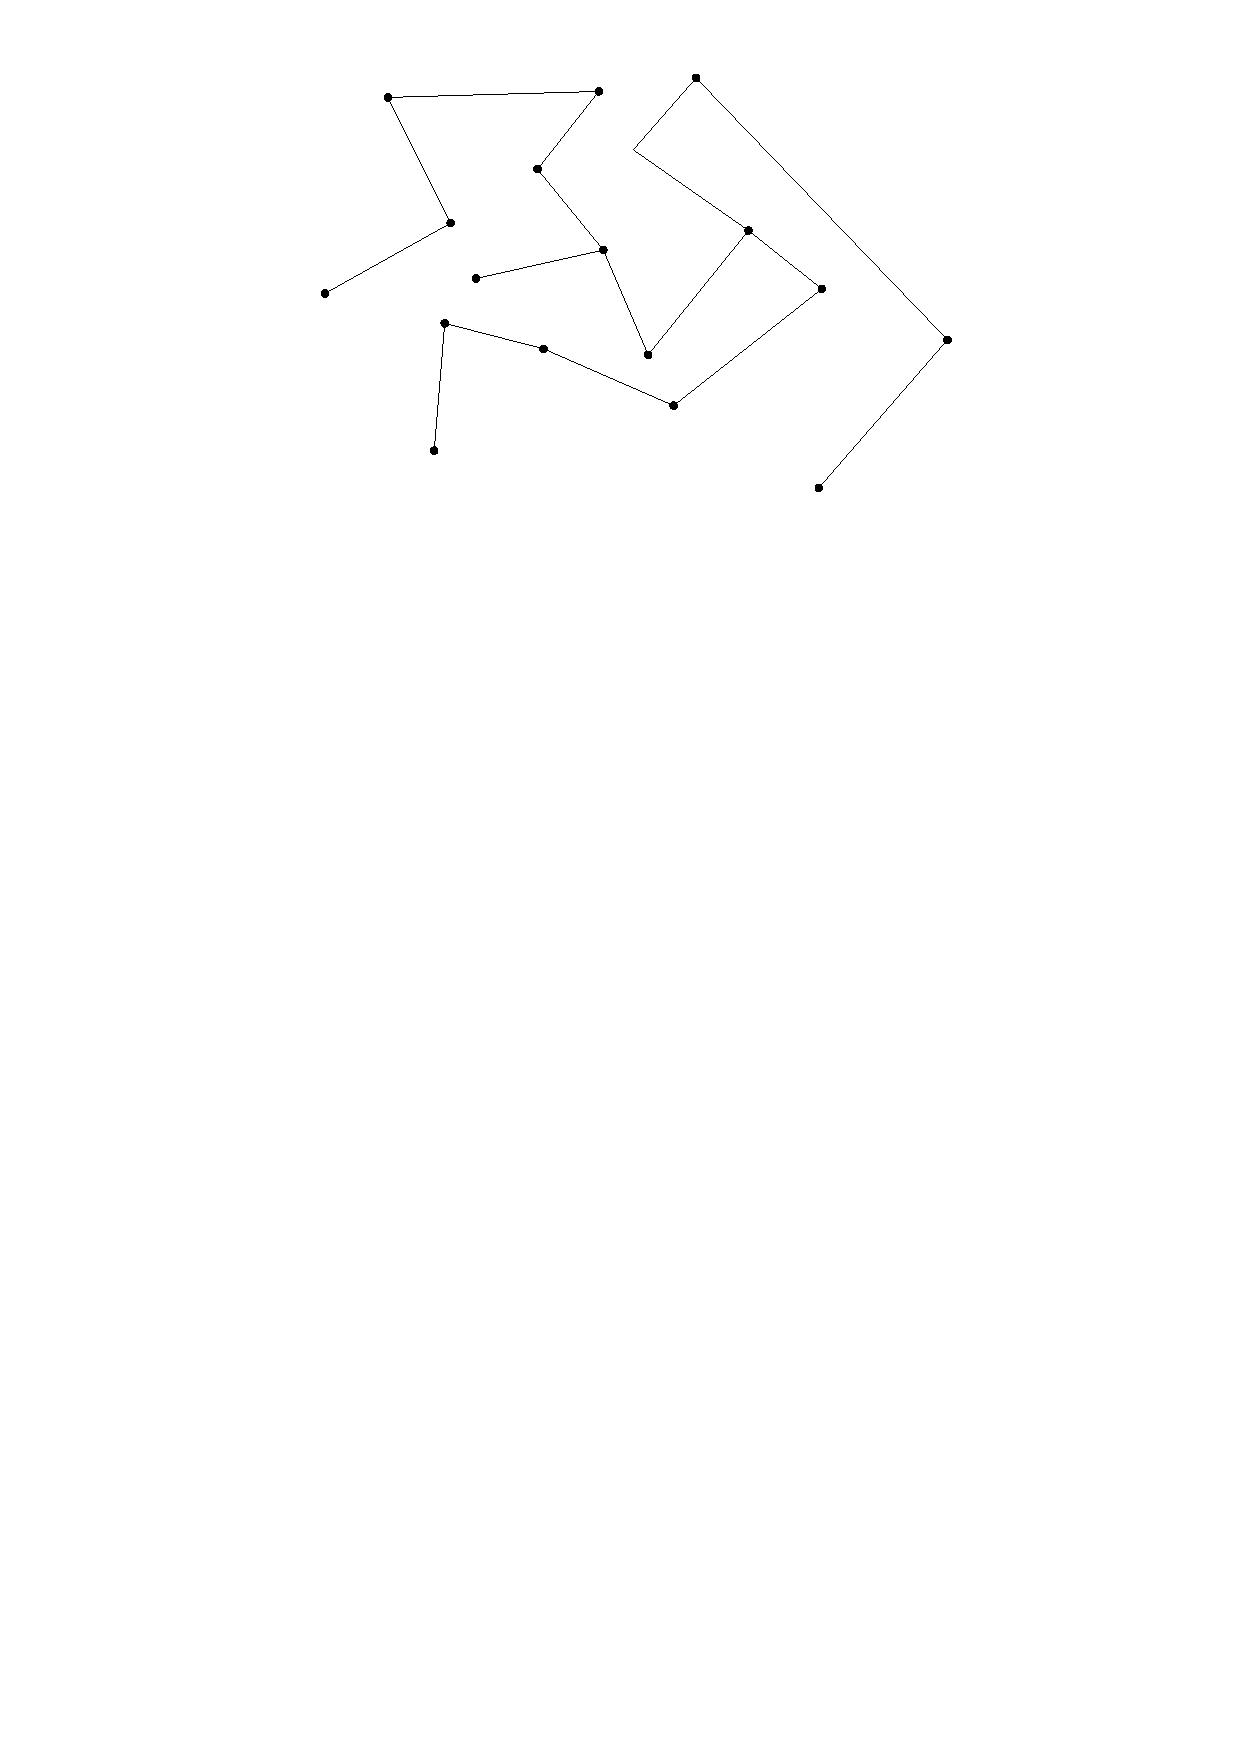
\includegraphics[scale=.5]{graphics/randomLinkage.pdf}
% \end{center} 
% \caption{A linkage with joints.}
% \end{figure} 
% \begin{figure}[h]
% \begin{center}
% 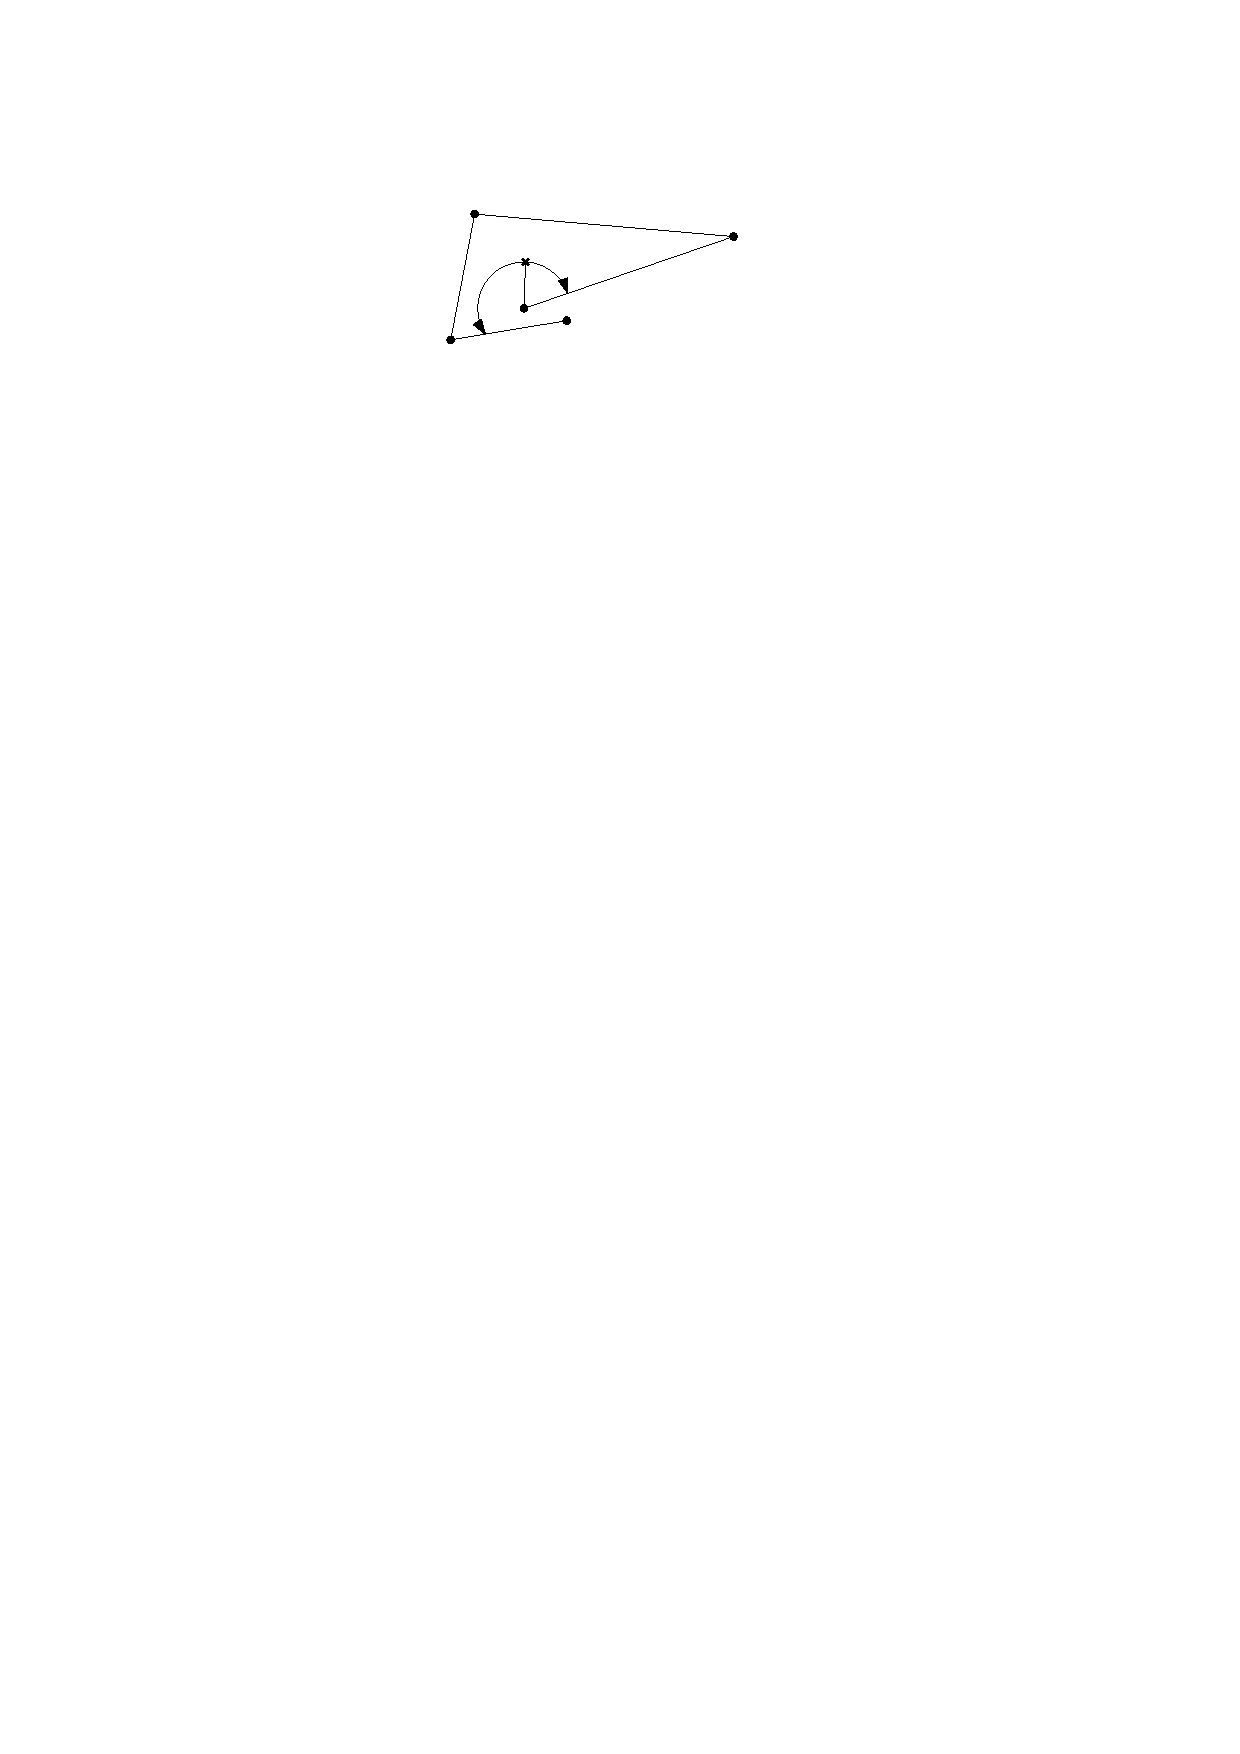
\includegraphics{graphics/freeJointPinnedJoint.pdf}
% \end{center} 
% \caption{The cross represents a free joint; the pinned joints are denoted as disks.  The range of motion shown by the arc describes the continous configuration space of the linkage.}
% \end{figure} 
% 
% For illustrations in the remainder of this paper, free joints will be represented as crosses and pinned joints will be represented as disks.
